\documentclass[a4paper,11pt]{article}
\usepackage[utf8]{inputenc}
\usepackage{algorithmic}
\usepackage{algorithm}
\usepackage{pst-plot}
\usepackage{graphicx}
\usepackage{endnotes}
\usepackage{graphics}
\usepackage{floatflt}
\usepackage{wrapfig}
\usepackage{amsfonts}
\usepackage{amsmath}
\usepackage{verbatim}
\usepackage{hyperref}
\usepackage{multirow}
\usepackage{pdflscape}
 \usepackage{enumitem}

\usepackage{hyperref}
\hypersetup{pdfborder={0 0 0 0}}

\pdfpagewidth 210mm
\pdfpageheight 297mm 
\setlength\topmargin{0mm}
\setlength\headheight{0mm}
\setlength\headsep{0mm}
\setlength\textheight{250mm}	
\setlength\textwidth{159.2mm}
\setlength\oddsidemargin{0mm}
\setlength\evensidemargin{0mm}
\setlength\parindent{7mm}
\setlength\parskip{0mm}

\newenvironment{exercise}[3]{\paragraph{Exercise #1: #2 (#3pt)}\ \\}{
\medskip}
\newcommand{\question}[2]{\setlength\parindent{0mm}\ \\$\mathbf{Q_#1:}$ #2\ \\}

\author{\large{Ilya Kuzovkin, Raul Vicente}}
\title{\huge{Introduction to Computational Neuroscience}\\\LARGE{Practice Session on Machine Learning}}

\begin{document}
\maketitle


%
% Intro
%
The main purpose of the field of \emph{neural decoding} is to reconstruct stimuli that led to the neuronal response presented in the data. Usually we have a finite set of stimuli and we show them to the test subjects. And in the same time we record responses on the test subject's brain. The task is to create a \emph{model}, which takes piece of recorded data as an input and \emph{predicts} which stimulus is responsible for producing this piece of data.

In the practice session on spiking data we attempted to \emph{manually} create one such model: by looking at the firings of 72 neurons we identified the stimulus (orientation of the bar on the screen). Although such approach can be very fruitful, it is often impossible to embrace all of the data manually. The data can be too massive or too complex or it can be hard to find an intuition, which would explain features of the data.

Here the field of \emph{machine learning} comes in. The main goal of machine learning can be summarized as providing an automatic way of finding dependencies between the data and the stimuli.\\


%
% ML introduction
%
\ \\
Before we continue let us go through vocabulary:
\begin{itemize}
\itemsep 0em
	\item \textbf{Dataset} is a structure which contains all the data we have.
	\item Dataset consist of \textbf{instances}. For example 4500ms of spiking data recorded while showing one stimulus is an instance.
	\item Instances consist of \textbf{features}. Those are parameters, which describe our data. For example average spiking rate is a feature, SPTH distribution is a feature, etc. Each instance has its own values of the features: for example one trial has spiking rate of 7 spikes/second, while another trial has spiking rate of 23 spikes/second.
	\item All features put together form a \textbf{feature vector}.
	\item One feature vector is a representation of one instance in the \textbf{feature space}. All instances live in there.
	\item Each instance belongs to a certain \textbf{class}. In previous dataset we had 12 different orientations, so each one represents different class in our dataset.
	\item The goal of a machine learning algorithm is to create a \textbf{model}, which can \textbf{classify} previously unseen data. For example we show one of the stimuli to the mouse, record new 4500ms of data, give this data to the model and the model tells us which stimulus was shown.
	\item The model is created from examples. Those are instances for which the class is known. Set of such examples is called \textbf{training set}, because we train our model on it.
	\item \textbf{Test set} is another set of instances, for which we also know the true class, but we do not give it to the model. We give the data (without the class) to the model and we ask the model to guess the class of the each instance.
	\item We can see how many instances from the test set model has identified correctly and the rate $$\displaystyle\frac{\text{Number of correctly classified instances}}{\text{Total number of instances}}$$ is called \textbf{accuracy}\footnote{Accuracy is a naive way to measure performance of the model. Read about \emph{precision} and \emph{recall} here \url{http://en.wikipedia.org/wiki/Precision_and_recall}} and it used to evaluate model's performance.
\end{itemize}


%
% Questions
%
\begin{exercise}{1}{Few questions}{0.5}
\question{1}{Why do you need to separate training and test datasets, that is why can't you evaluate your model on the training set?}
\question{2}{Let us say that you have 2 classes and your model predicts the class correctly in 50\% of the cases. How useful this model is?}
\question{3}{What does it mean if your model's accuracy on the training set is high, but on the test set it is very low?}
\question{4}{Imagine we have a classification problem with 2 classes: 0 and 1. And imagine we have a very stupid predictive model which always predicts 1. Can you come up with such a test set, for which this predictive model will yield high accuracy, say 0.9?}
\end{exercise}



%
% fMRI
%
\begin{exercise}{2}{Which picture was shown?}{2.5}
\begin{wrapfigure}{r}{0.4\textwidth}
	\centering
	\vspace{-45pt}
	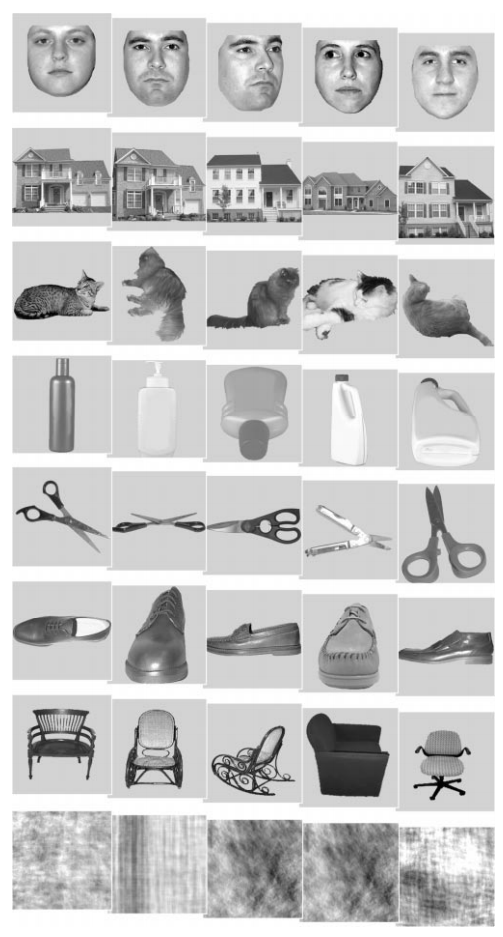
\includegraphics[width=0.35\textwidth]{stimuli.png}
	\caption{Examples of stimuli.}
	\label{fig:stimuli}
	\vspace{-20pt}
\end{wrapfigure}
In this session we will work with fMRI dataset\footnote{\url{https://openfmri.org/dataset/ds000105}} by Haxby et al.\footnote{\url{http://www.cs.pomona.edu/~syang/arch/visual_decoding/haxby_2001pdf.pdf}}. The data was recorded while test subject was presented with images from 9 categories: (1) house,  (2) scrambled, (3) cat, (4) shoe, (5), bottle, (6) scissors, (7) chair, (8) face, (9) something else. You can see them (except for the ``something else" category) on the Figure \ref{fig:stimuli}. The data we have is already preprocessed, so instead of $\approx$25000 voxels we have 577. In machine learning terminology this means that each instance has 577 features and belongs to one of the 9 classes. You will find the feature data in \texttt{data/voxels.mat} and class information \texttt{data/labels.mat}. First one is 1492$\times$577 matrix (1492 instances 577 features each) and the second one is a vector of length 1492 (each instance has a class).

The question we want to answer is: \emph{Is is possible to detect from the fMRI signal the image the test subject was looking at?}. Your task will be to use Matlab \texttt{classify}\footnote{http://se.mathworks.com/help/stats/classify.html} function to build a predictive model. We will not go into the details of how exactly machine learning algorithm behind it works. For that I recommend taking a Machine Learning course.

Perform the following steps and report the results:
\begin{enumerate}
	\item Load the data.
	\item Split data into training and test set (take 1000 instances for training and 492 for testing).
	\item Read carefully \texttt{classify} function manual.
	\item Use training set to train a model and with that model predict the classes of the test set.
	\item For each class compare the predicted class and the true class and report the accuracy for each class separately.
\end{enumerate}
\end{exercise}


%
% Confusion matrix
%
\begin{exercise}{3}{Confusion matrix}{1}
Accuracies alone do not give you full overview of where exactly your model goes wrong. A nice way to visualize your model's performance is to build so called \emph{confusion matrix}. Rows of this matrix are true classes and the columns are the predicted classes. So for example cell on the intersection of the row \#2 and column \#4 shows how many instances of class 2 were classified as class 4. Construct a confusion matrix for the results of the previous exercise.
\end{exercise}


%
% Precision and Recall
%
\begin{exercise}{4}{Precision, Recall, F1-score}{1}
In the 4th question of the first exercise we've seen how accuracy can fail us if we are dealing with unbalanced datasets. One possible countermeasure is to look not at the accuracy of the model, but at its \emph{precision} and \emph{recall}. 
Imagine you have 2 classes: ``cat" and ``non-cat". Precision is calculated for each class separately and shows how many of the instances the model has identified as cats are really cats. For example if out of 10 instances classified as ``cats" two turn out to be ``non-cats" we say that precision is 0.8.
Recall is also calculated separately for each class. It shows how many of all cats present in the dataset your model has identified as such. For example if there were 100 cats and 100 non-cats and our models correctly identified 78 cats we say that its recall is 0.78.
F1 score is a convenient metric to write precision and recall as one number:
$$F1 = 2 \cdot \frac{\text{precision} \cdot \text{recall}}{\text{precision} + \text{recall}}$$
Your task is to calculate precision, recall and f1-score for each of 9 classes.
\end{exercise}


\begin{exercise}{5*}{Cross-validation}{1}
In the second exercise we've separated our data into training set and test set. We took first 1000 as training and the rest as test. You might wonder would the results be different if we would take first 500 instances as test and the rest as training, or middle 500 as test and the rest as training. And this is a very good question to ask: indeed, maybe we just got lucky with our particular selection of instances in the test set and if we choose other, then scores will be lower. To resolve this issue and answer that question you need to use a technique called \emph{cross-validation}:
\begin{enumerate}
	\item Split our data into 10 sets\footnote{This is called \emph{10-fold cross-validation.}} $S_1, S_2, ... S_{10}$ of equal size.
	\item For each set $S_i$:
	\begin{enumerate}
		\item Train a model on all data from sets $S_1, ..., S_{i-1}, S_{i+1}, ... S_{10}$
		\item Test the model on set $S_i$
	\end{enumerate}
	\item Report average F1 score for each class.
\end{enumerate}
\end{exercise}
\ \\
\ \\
\ \\
\ \\
\ \\
Please submit a \texttt{pdf} report with answers to the questions and comments about your solutions. Include figures, explanations and essential pieces of code. Do not include the code itself as a separate file, your report should give good understanding of what you have done. Please mark how long it took to complete this set of exercises. Upload the \texttt{pdf} to the practice session page on the course website.

\end{document}










